\documentclass[a4paper,11pt,russian]{extreport}
% Эта строка — комментарий, она не будет показана в выходном файле
\usepackage[T2A]{fontenc}
\usepackage[utf8]{inputenc} % Включаем поддержку UTF8
\usepackage[russian]{babel}%используем русский и английский языки с переносами
\usepackage{enumerate}
\usepackage{etoolbox}
\usepackage{amsmath}
\usepackage{listings}
\usepackage{pgfplots}
\usepackage{pgfplotstable}
\pgfplotsset{every axis legend/.append style={
		at={(1,1)},
		anchor=north west}}


\usepackage{titlesec}
\titleformat{\chapter}[block]
{\Huge\bfseries}{\thechapter}{10pt}{\Huge}

\usepackage[left=3cm,right=3cm,
top=2cm,bottom=2cm]{geometry}

\lstset{numbers=left}

\newcommand*{\No}{\textnumero}

\begin{document}
	\begin{titlepage}
		\begin{center} 
			Государственное образовательное учреждение высшего профессионального образования
			
			
			«Московский Государственный Технический Университет имени Н. Э. Баумана»
		\end{center}
		\vspace*\fill
		\begin{center}
			\scshape\LARGE {
				Отчет по лабораторной работе \No 1\\
				<<Гистограмма и эмпирическая функция распределения>> \\
				по курсу <<Математическая статистика>>\\
				}
			\scshape\Large{Вариант 1 \\}
			\vspace{1cm}
			\scshape\Large{
				Студент: Анисимов Н.С. ИУ7-62 \\
				Преподаватель: Велищанский М.А.\\ }
			
		\end{center}
		\vspace*\fill
		\centering\today
	\end{titlepage}
	
	\tableofcontents
	
	\newpage
	
	\chapter{Формулы и определения}
	
	\section{Формулы}
	
	\paragraph{Минимальное значение выборки}
	
	
	\begin{equation}
	M_{\min} = \min \{ x_1, \dots, x_n\}
	\end{equation}
	\begin{itemize}
		\item $(x_1, \dots, x_n)$ --- реализация случайной выборки.
	\end{itemize}
	
	
	\paragraph{Максимальное значение выборки}
	
	\begin{equation}
	M_{\max} = \max \{ x_1, \dots, x_n\}
	\end{equation}
	\begin{itemize}
		\item $(x_1, \dots, x_n)$ --- реализация случайной выборки.
	\end{itemize}
	
	
	\paragraph{Размах выборки}
	
	\begin{equation}
	R = M_{\max} - M_{\min}
	\end{equation}
	\begin{itemize}
		\item $M_{\max}$ --- максимальное значение выборки;
		\item $M_{\min}$ --- минимальное значение выборки.
	\end{itemize}
	
	
	\paragraph{Оценка математического ожидания}
	
	\begin{equation}
	\hat{\mu}(\vec{x}_n) =\frac{1}{n} \sum_{i = 1}^{n} x_i
	\end{equation}
	
	
	\paragraph{Смещённая оценка дисперсии}
	
	\begin{equation}
	\hat{\sigma}^2(\vec{x}_n) = \frac{1}{n} \sum_{i = 1}^{n}(x_i - \hat{\mu})^2
	\end{equation}
	
	
	\paragraph{Несмещённая оценка дисперсии}
	
	\begin{equation}
	S^2(\vec{x}_n) = \frac{n}{n - 1}\hat{\sigma}^2 = \frac{1}{n - 1}\sum_{i = 1}^{n}(x_i - \hat{\mu})^2
	\end{equation}
	
	\iffalse
	\paragraph{Оценки для интервального ряда}
		
	\begin{equation}
	\hat{\sigma}^2(\vec{x}_n) = \frac{1}{n} \sum_{i = 1}^{n}n_{i}\frac{x_{(1)}+(i-1)\Delta+x_{(1)}+i\Delta}{2}
	\end{equation}
	
	\begin{equation}
	\hat{\sigma}^2(\vec{x}_n) = \frac{1}{n} \sum_{i = 1}^{n}n(\frac{x_{(1)}+(i-1)\Delta+x_{(1)}+i\Delta}{2} - \hat{\mu})^2
	\end{equation}
	
	
	\begin{equation}
	\hat{\sigma}^2(\vec{x}_n) = \frac{1}{n-1} \sum_{i = 1}^{n}n(\frac{x_{(1)}+(i-1)\Delta+x_{(1)}+i\Delta}{2} - \hat{\mu})^2
	\end{equation}
	
	\begin{itemize}
		\item $n_{i}$ --- число элементов выборки $\vec{x}$, которые попали в интервал $J_{i}$;
		\item $n$ --- объем выборки;
		\item $\Delta$ --- $\frac{x_{n}-x_{1}}{m}$ , где $m \in N$ число интервалов;
		\item $J_{i}=[x_{(1)}+(i-1)\Delta;\ x_{(1)}+i\Delta), i = \overline{1;m-1}$;
		\item $J_{m}=[x_{(1)}+(m-1)\Delta;\ x_{(n)}], i = \overline{1;m-1}$.
	\end{itemize}
	\fi
	
	\section{Определение эмпирической плотности и гистограммы}
	Эмпирической плотностью распределения, соответствующей выборке $\vec{x}$, называется функция:
	
	\begin{equation}
	f_n(x) = \begin{cases} \frac{n_i}{n\Delta}, & x \in J_i \\ 0, & x \notin \bigcup\limits_{i=1}^{m}J_i \end{cases}
	\end{equation}
	
	\begin{itemize}
		\item $n_{i}$ --- число элементов выборки $\vec{x}$, которые попали в интервал $J_{i}$;
		\item $n$ --- объем выборки;
	\end{itemize}
	График функции $f_n(x)$ называется гистограммой.
	
	\section{Определение эмпирической функции распределения}
	Пусть $\vec{X}=(X_1, \dots , X_n)$ – случайная выборка, $\vec{x}=(x_1, \dots , x_n)$ – реализация этой случайной выборки. Обозначим $n(x,\vec{x})$ – количество элементов вектора $\vec{x}$, которые меньше $x$.
	
	Эмпирической функцией распределения, построенной по выборке $\vec{x}$, называют отображение $F_n\colon \Re \to \Re$, определенное правилом:
	
	\begin{equation}
	F_n(x) = \frac{n(x, \vec{x})}{n}
	\end{equation}
	
	\chapter{Листинг}
	\lstinputlisting[language=MatLab]{../src/l1.m}
	
	\chapter{Результаты}
	\begin{align*}
	M_{\min} =& -4.110000 \\
	M_{\max} =& 1.400000 \\
	R =& 5.510000 \\
	\hat{\sigma}^2 =& -1.604583 \\
	S^2 =& 1.034091
	\end{align*}
	Интервальный статистический ряд \\
	\begin{align*}
	[-4.110000;\ -3.421250)\quad & 4 \\
	[-3.421250;\ -2.732500)\quad & 11 \\
	[-2.732500;\ -2.043750)\quad & 26 \\
	[-2.043750;\ -1.355000)\quad & 33 \\
	[-1.355000;\ -0.666250)\quad & 26 \\
	[-0.666250;\ 0.022500)\quad & 15 \\
	[0.022500;\ 0.711250)\quad & 2 \\
	[0.711250;\ 1.400000]\quad & 3
	\end{align*}
	
	\begin{figure}
		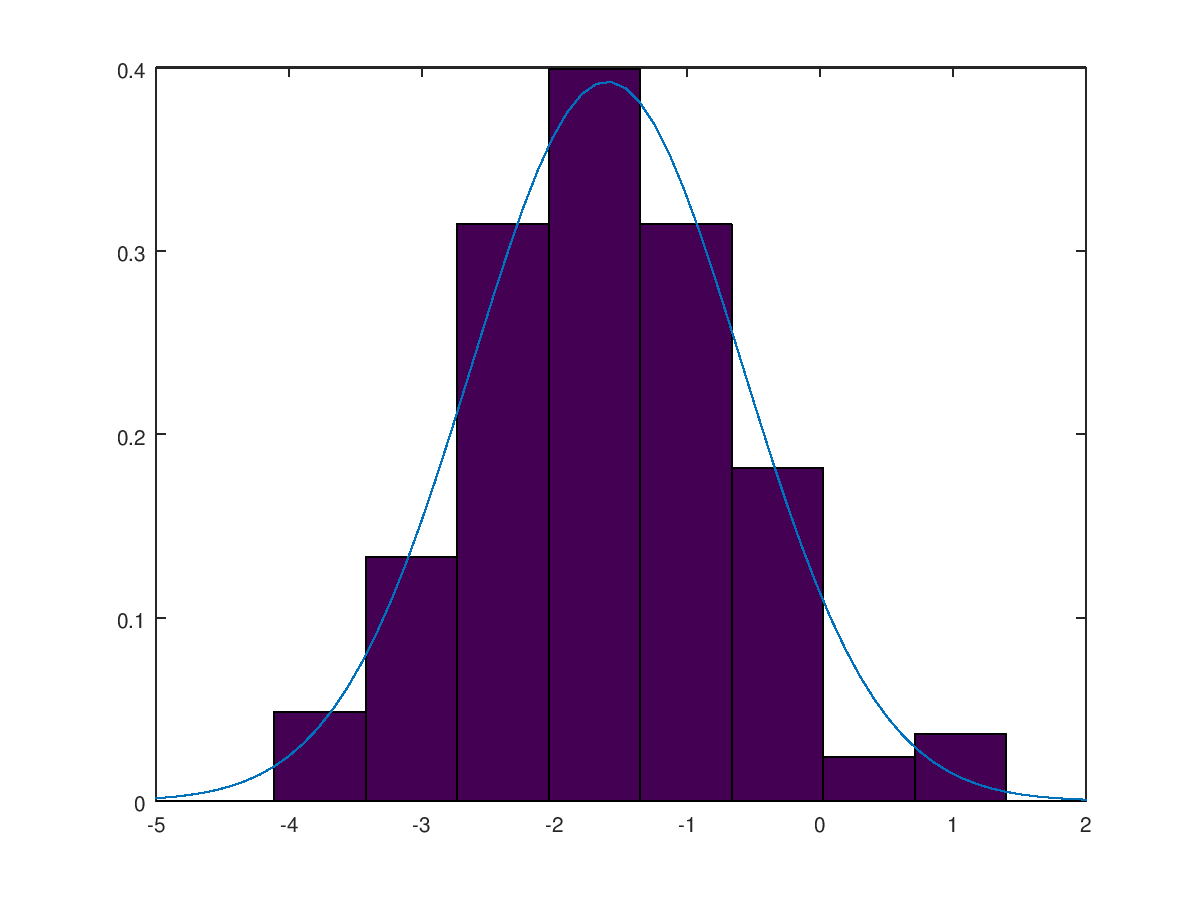
\includegraphics[width=\linewidth]{../img/1.png}
		\caption{Гистограмма и график функции плотности распределения вероятностей нормальной случайной величины}
		\label{fig:1}
	\end{figure}
	
	\begin{figure}
		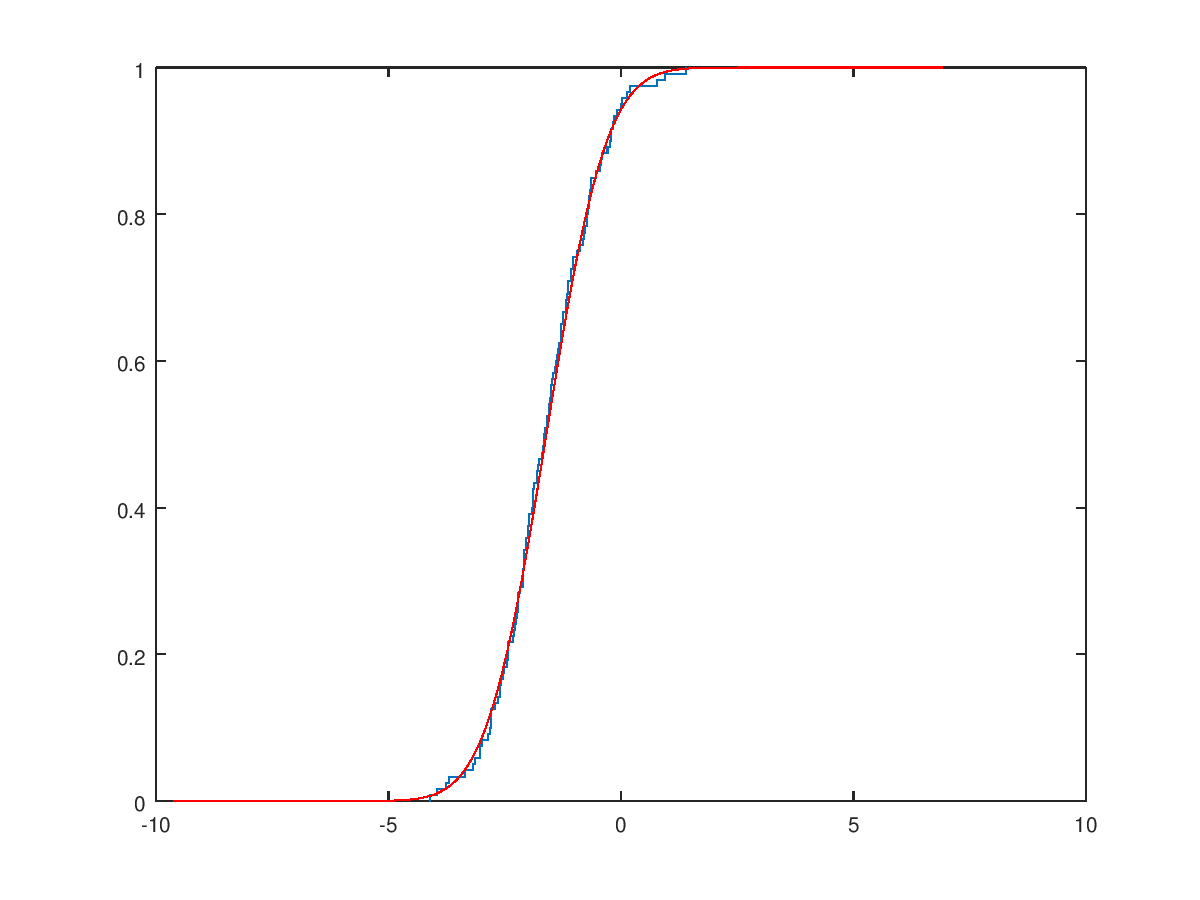
\includegraphics[width=\linewidth]{../img/2.png}
		\caption{Графики эмпирической функции распределения и функции распределения нормальной случайной величины}
		\label{fig:2}
	\end{figure}
	
		
	
\end{document}